\setbeamercolor{background canvas}{bg=white}
\color{black}


\begin{frame}
    \transfade
    
\begin{textblock}{14}(1,2)
\begin{itemize}
        \item<1-> 
        For every edge in a DAG, the starting vertex is visited before ending vertex..
\end{itemize}
\end{textblock}


\begin{textblock}{16}(0,4)
    \begin{figure}
    \centering
    \begin{tikzpicture}
    \node<2> (a) [inactive node] {a} ;
    \node<2> (b) [inactive node, right of = a, xshift = 40, yshift = 50] {b};
    \node<2> (c) [inactive node, right of = a, xshift = 40, yshift = -50] {c};
    
    \draw<2> [inactive edge] (a) -- (b);
    \draw<2> [inactive edge] (a) -- (c);
    \draw<2> [inactive edge] (b) -- (c);
    
    \end{tikzpicture}
\end{figure}
\end{textblock}






   
\end{frame}
\begin{frame}
    \transfade
    \begin{textblock}{14}(1,2)
\begin{itemize}
        \item<1-> 
        For every edge in a DAG, the starting vertex is visited before ending vertex..
\end{itemize}
\end{textblock}


\begin{textblock}{16}(0,4)
    \begin{figure}
    \centering
    \begin{tikzpicture}
    \node<1-> (a) [active node] {a} ;
    \node<1-> (b) [active node, right of = a, xshift = 40, yshift = 50] {b};
    \node<1-> (c) [inactive node, right of = a, xshift = 40, yshift = -50] {c};
    
    \draw<1-> [active edge] (a) -- (b);
    \draw<1-> [inactive edge] (a) -- (c);
    \draw<1-> [inactive edge] (b) -- (c);
    
    \end{tikzpicture}
\end{figure}
\end{textblock}


\begin{textblock}{14}(1,9)
    \begin{itemize}
        \item<2> a is visited before b 
    \end{itemize}
    
\end{textblock}
   
\end{frame}
\begin{frame}
    \transfade
    \begin{textblock}{14}(1,2)
\begin{itemize}
        \item<1-> 
        For every edge in a DAG, the starting vertex is visited before ending vertex..
\end{itemize}
\end{textblock}


\begin{textblock}{16}(0,4)
    \begin{figure}
    \centering
    \begin{tikzpicture}
    \node<1-> (a) [active node] {a} ;
    \node<1-> (b) [inactive node, right of = a, xshift = 40, yshift = 50] {b};
    \node<1-> (c) [active node, right of = a, xshift = 40, yshift = -50] {c};
    
    \draw<1-> [inactive edge] (a) -- (b);
    \draw<1-> [active edge] (a) -- (c);
    \draw<1-> [inactive edge] (b) -- (c);
    
    \end{tikzpicture}
\end{figure}
\end{textblock}


\begin{textblock}{14}(1,9)
    \begin{itemize}
        \item<2> a is visited before c 
    \end{itemize}
    
\end{textblock}
   
\end{frame}
\begin{frame}
    \transfade
    \begin{textblock}{14}(1,2)
\begin{itemize}
        \item<1-> 
        For every edge in a DAG, the starting vertex is visited before ending vertex..
\end{itemize}
\end{textblock}


\begin{textblock}{16}(0,4)
    \begin{figure}
    \centering
    \begin{tikzpicture}
    \node<1-> (a) [inactive node] {a} ;
    \node<1-> (b) [active node, right of = a, xshift = 40, yshift = 50] {b};
    \node<1-> (c) [active node, right of = a, xshift = 40, yshift = -50] {c};
    
    \draw<1-> [inactive edge] (a) -- (b);
    \draw<1-> [inactive edge] (a) -- (c);
    \draw<1-> [active edge] (b) -- (c);
    
    \end{tikzpicture}
\end{figure}
\end{textblock}


\begin{textblock}{14}(1,9)
    \begin{itemize}
        \item<2> b is visited before c 
    \end{itemize}
    
\end{textblock}
   
\end{frame}

\setbeamercolor{background canvas}{bg=black}
\begin{frame}{}
    \transcover
\begin{tikzpicture}
    \draw[color=white,fill=white,transform canvas={xshift = 5cm, yshift=-0.5cm}] (0,0) rectangle (0.2,3);
\end{tikzpicture}
\begin{textblock}{5}(6.5,7.3)
\fontfamily{qhv}\selectfont
\Huge\color{white} \textbf{WHY?}
\end{textblock}
\end{frame}
\setbeamercolor{background canvas}{bg=white}
\begin{frame}{}
    \transuncover
\end{frame}

\begin{frame}
    
    \transfade
   
    \begin{textblock}{16}(0,7)
        \centering
        \color{black}
        \Huge \textbf{Let's assemble a PC!!!}
    \end{textblock}
   
    
\end{frame}

\begin{frame}
    \transfade
    \color{black}



\begin{textblock}{16}(0,2)

\begin{figure}
    \centering
    \begin{tikzpicture}

\node[inner sep=0pt] (motherboard) at (3,0)
    {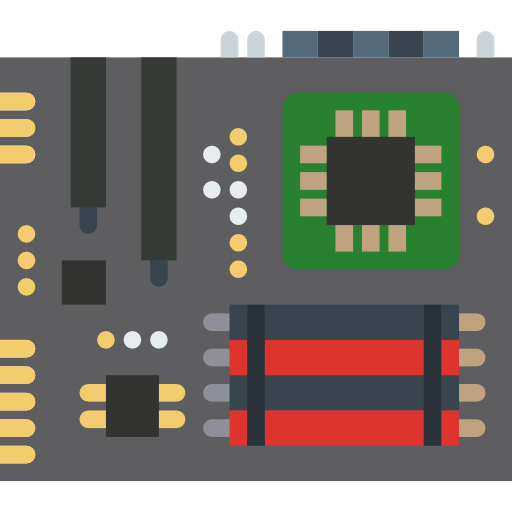
\includegraphics[width=.12\textwidth]{Simulation_sayem/pictures/motherboard.png}};  
\node[inner sep=0pt] (videocard) at (3,3)
    {
\includegraphics[width=.12\textwidth]{Simulation_sayem/pictures/video-card.png}};
    
\node[inner sep=0pt] (memory) at (0,0)
    {
\includegraphics[width=.12\textwidth]{Simulation_sayem/pictures/memory.png}};
    
\node[inner sep=0pt] (casing) at (6,0)
    {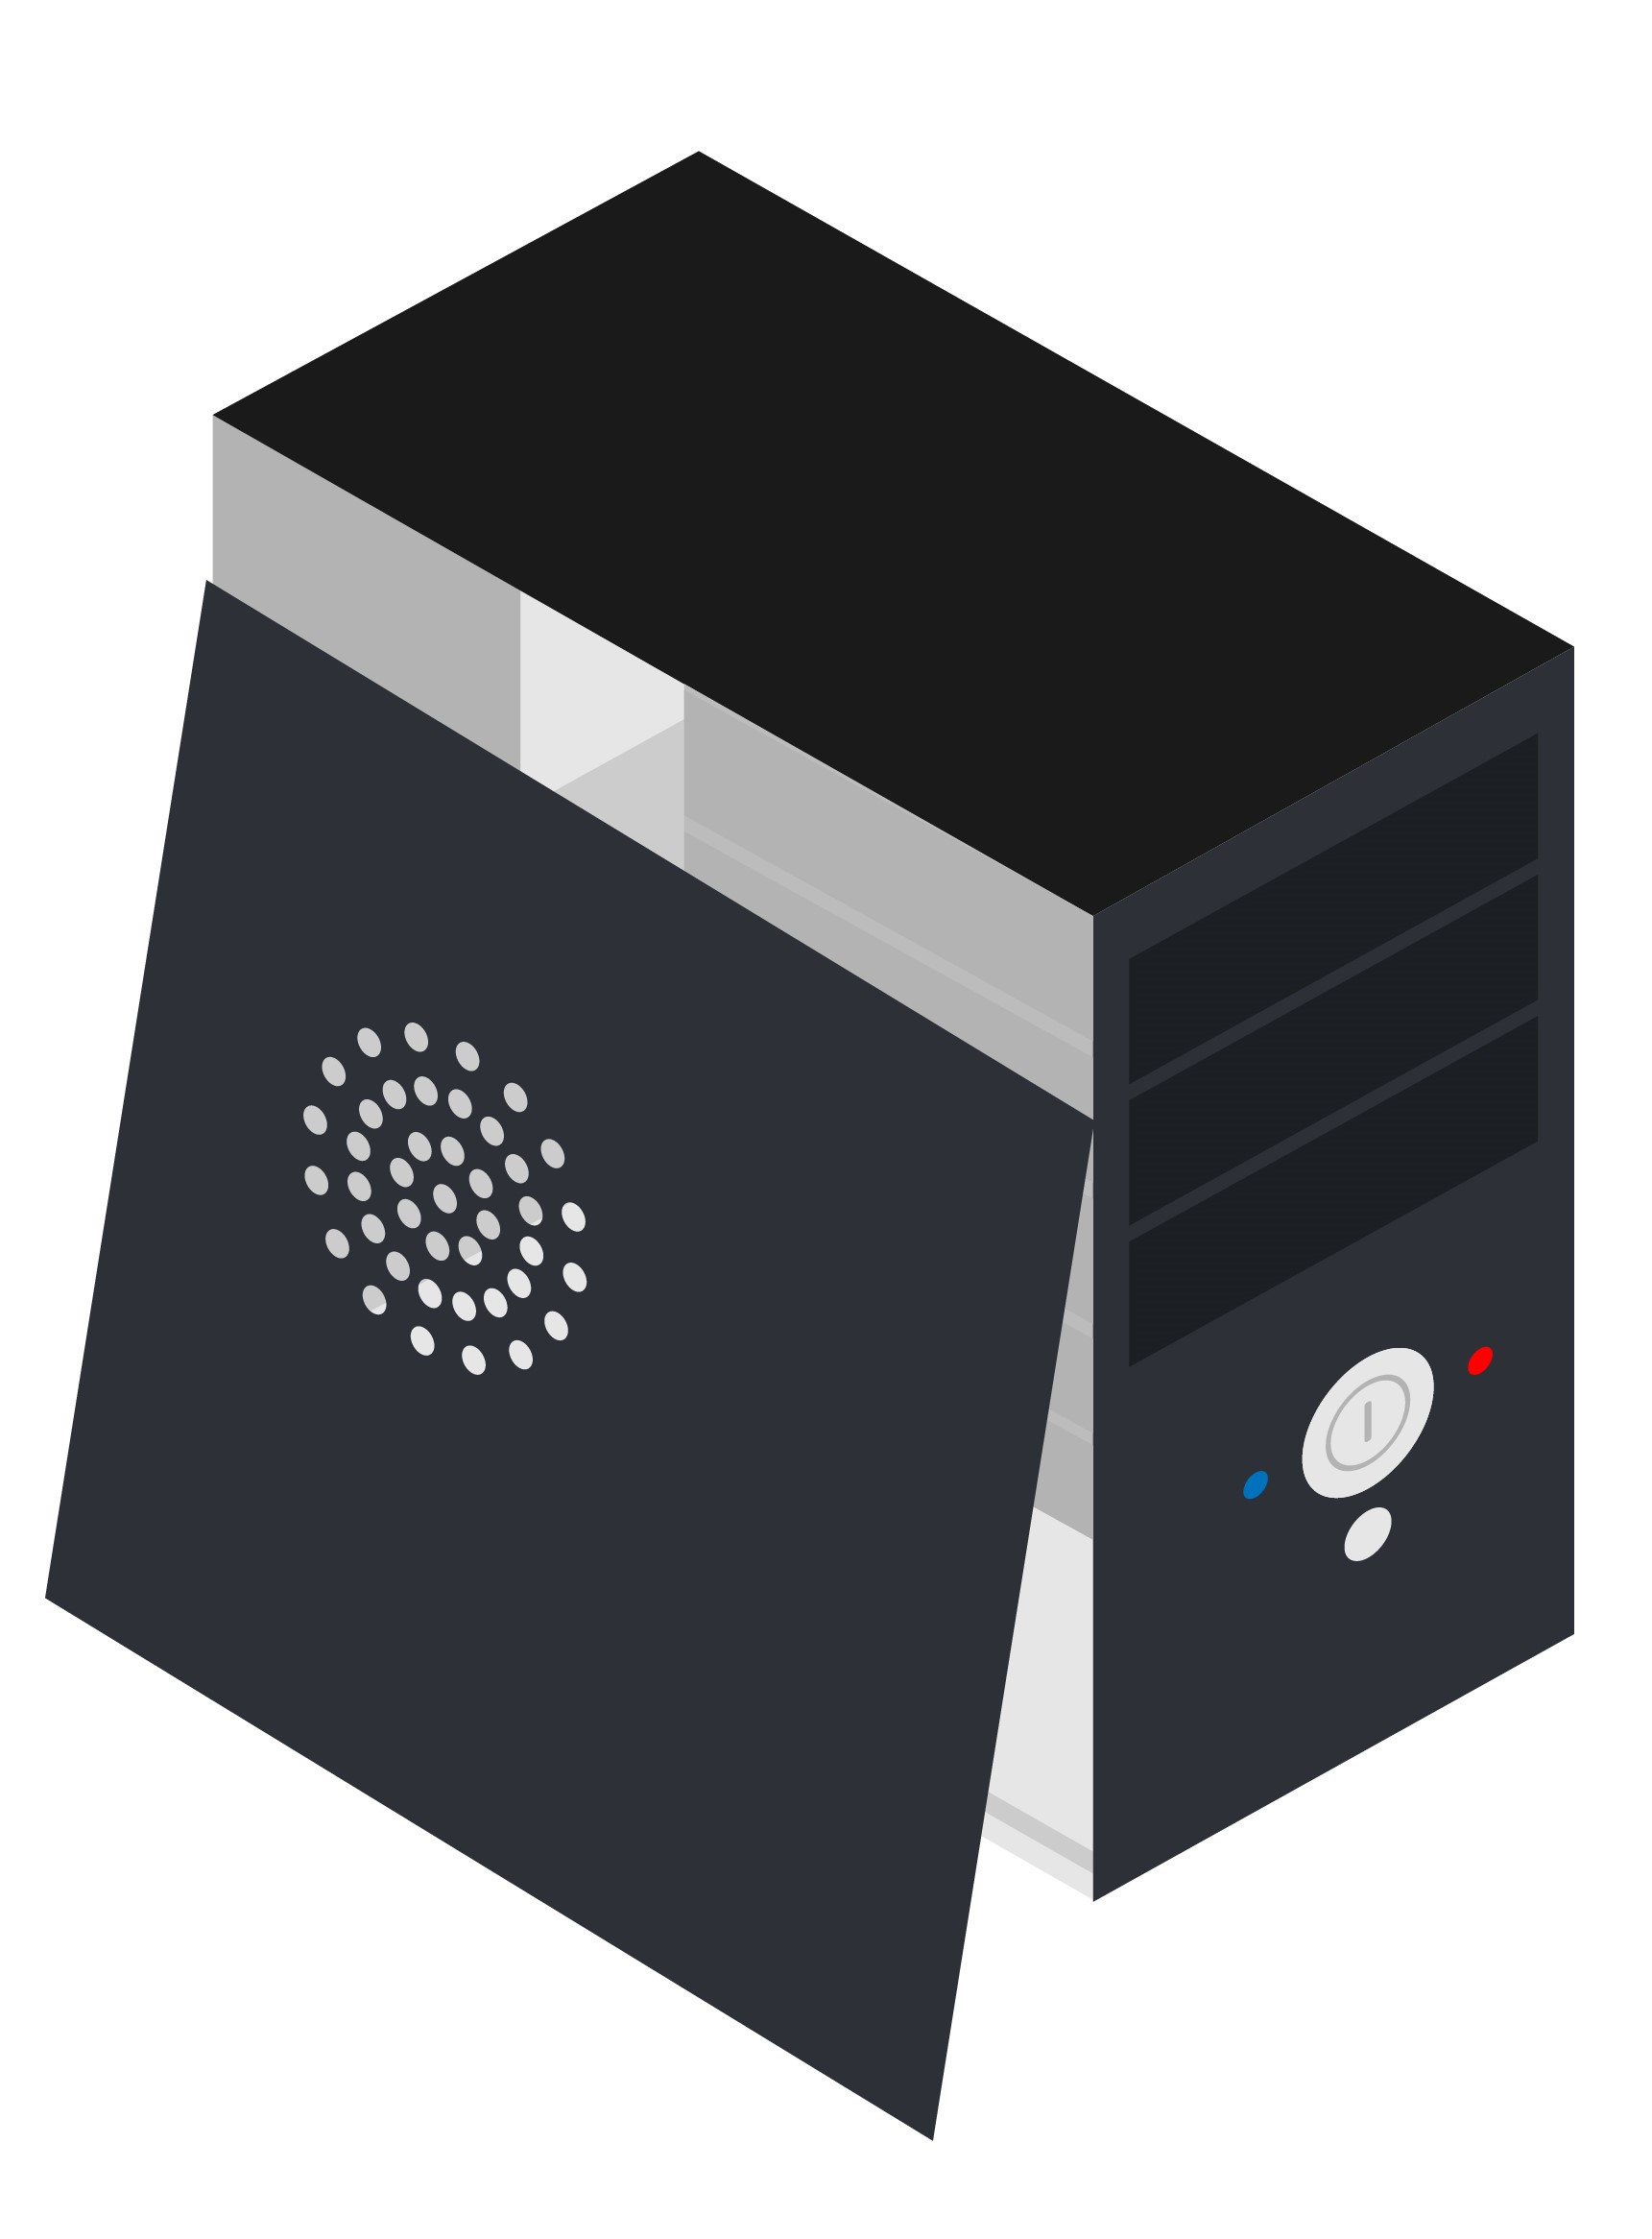
\includegraphics[width=.12\textwidth]{Simulation_sayem/pictures/casing.jpg}};
\node[inner sep=0pt] (PSU) at (6,3)
    {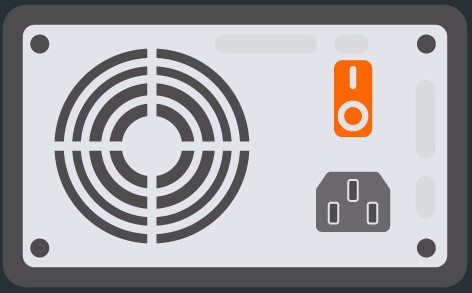
\includegraphics[width=.12\textwidth]{Simulation_sayem/pictures/powerSupply.jpg}};
\node[inner sep=0pt] (CPU) at (0,3) {
\includegraphics[width=.08\textwidth]{Simulation_sayem/pictures/processor.jpg}};


\node<3>[inner sep=0pt] (casingcross) at (6,0)
    {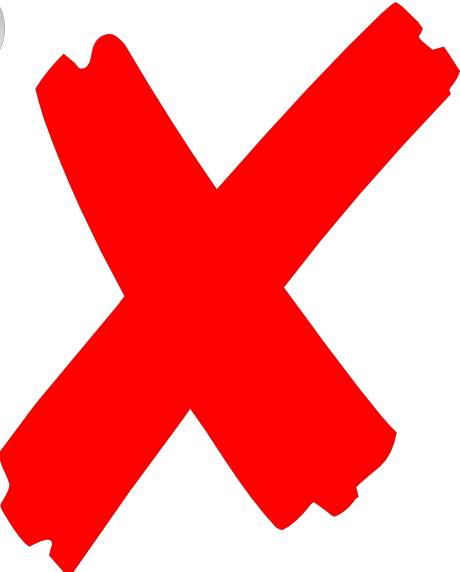
\includegraphics[width=.12\textwidth]{Simulation_sayem/pictures/cross.png}};
\node<6>[inner sep=0pt] (memorycross) at (0,0)
    {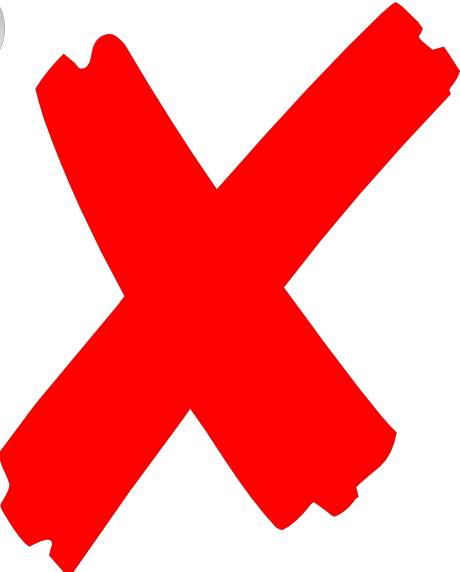
\includegraphics[width=.12\textwidth]{Simulation_sayem/pictures/cross.png}};


\draw<4-> [inactive edge] (PSU) --(casing);
\draw<4-> [inactive edge] (motherboard) --(casing);
\draw<10-> [inactive edge] (videocard) --(PSU);
\draw<8-> [inactive edge] (motherboard) --(videocard);
\draw<8-> [inactive edge] (CPU) --(videocard);
\draw<9-> [inactive edge] (motherboard) --(CPU);
\draw<7-> [inactive edge] (motherboard) --(memory);

\end{tikzpicture}
\end{figure}
\end{textblock}

\begin{textblock}{14}(5,12)
\begin{figure}
    \centering
    \begin{itemize}
        \only<2>{
        \vfill \item<2> Lets buy casing first }
        \only<3>{
        \vfill \item<3> But we can't!! }
        \only<4>{
        \vfill \item<4> We need motherboard and PSU model }
        \only<5>{
        \vfill \item<5> Lets try to buy RAM }
        \only<6>{
        \vfill \item<6> Again!! We can't }
        \only<7>{
        \vfill \item<7> We need motherboard model }
    \end{itemize}
\end{figure}
    
\end{textblock}
\end{frame}

\begin{frame}
    \transfade
    \begin{itemize}
        \item<1-> We can't buy things in random order
        \item<2-> Maintain the topological Order!!!
        
    \end{itemize}

\end{frame}

\begin{frame}
    \transfade
    \begin{textblock}{16}(0,6)
        \centering
        \color{black}
        \Large \textbf{Let's get back to our example}
    \end{textblock}
    
\end{frame}


\begin{frame}
    \transfade
    
\begin{textblock}{16}(0,2)
\begin{figure}
    \centering
    \begin{tikzpicture}

\node<1->[inner sep=0pt] (motherboard) at (3,0)
    {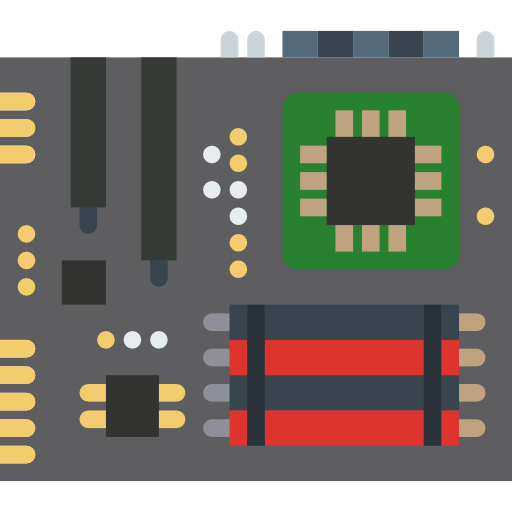
\includegraphics[width=.12\textwidth]{Simulation_sayem/pictures/motherboard.png}};  
\node<1->[inner sep=0pt] (videocard) at (3,3)
    {
\includegraphics[width=.12\textwidth]{Simulation_sayem/pictures/video-card.png}};
    
\node<1->[inner sep=0pt] (memory) at (0,0)
    {
\includegraphics[width=.12\textwidth]{Simulation_sayem/pictures/memory.png}};
    
\node<1->[inner sep=0pt] (casing) at (6,0)
    {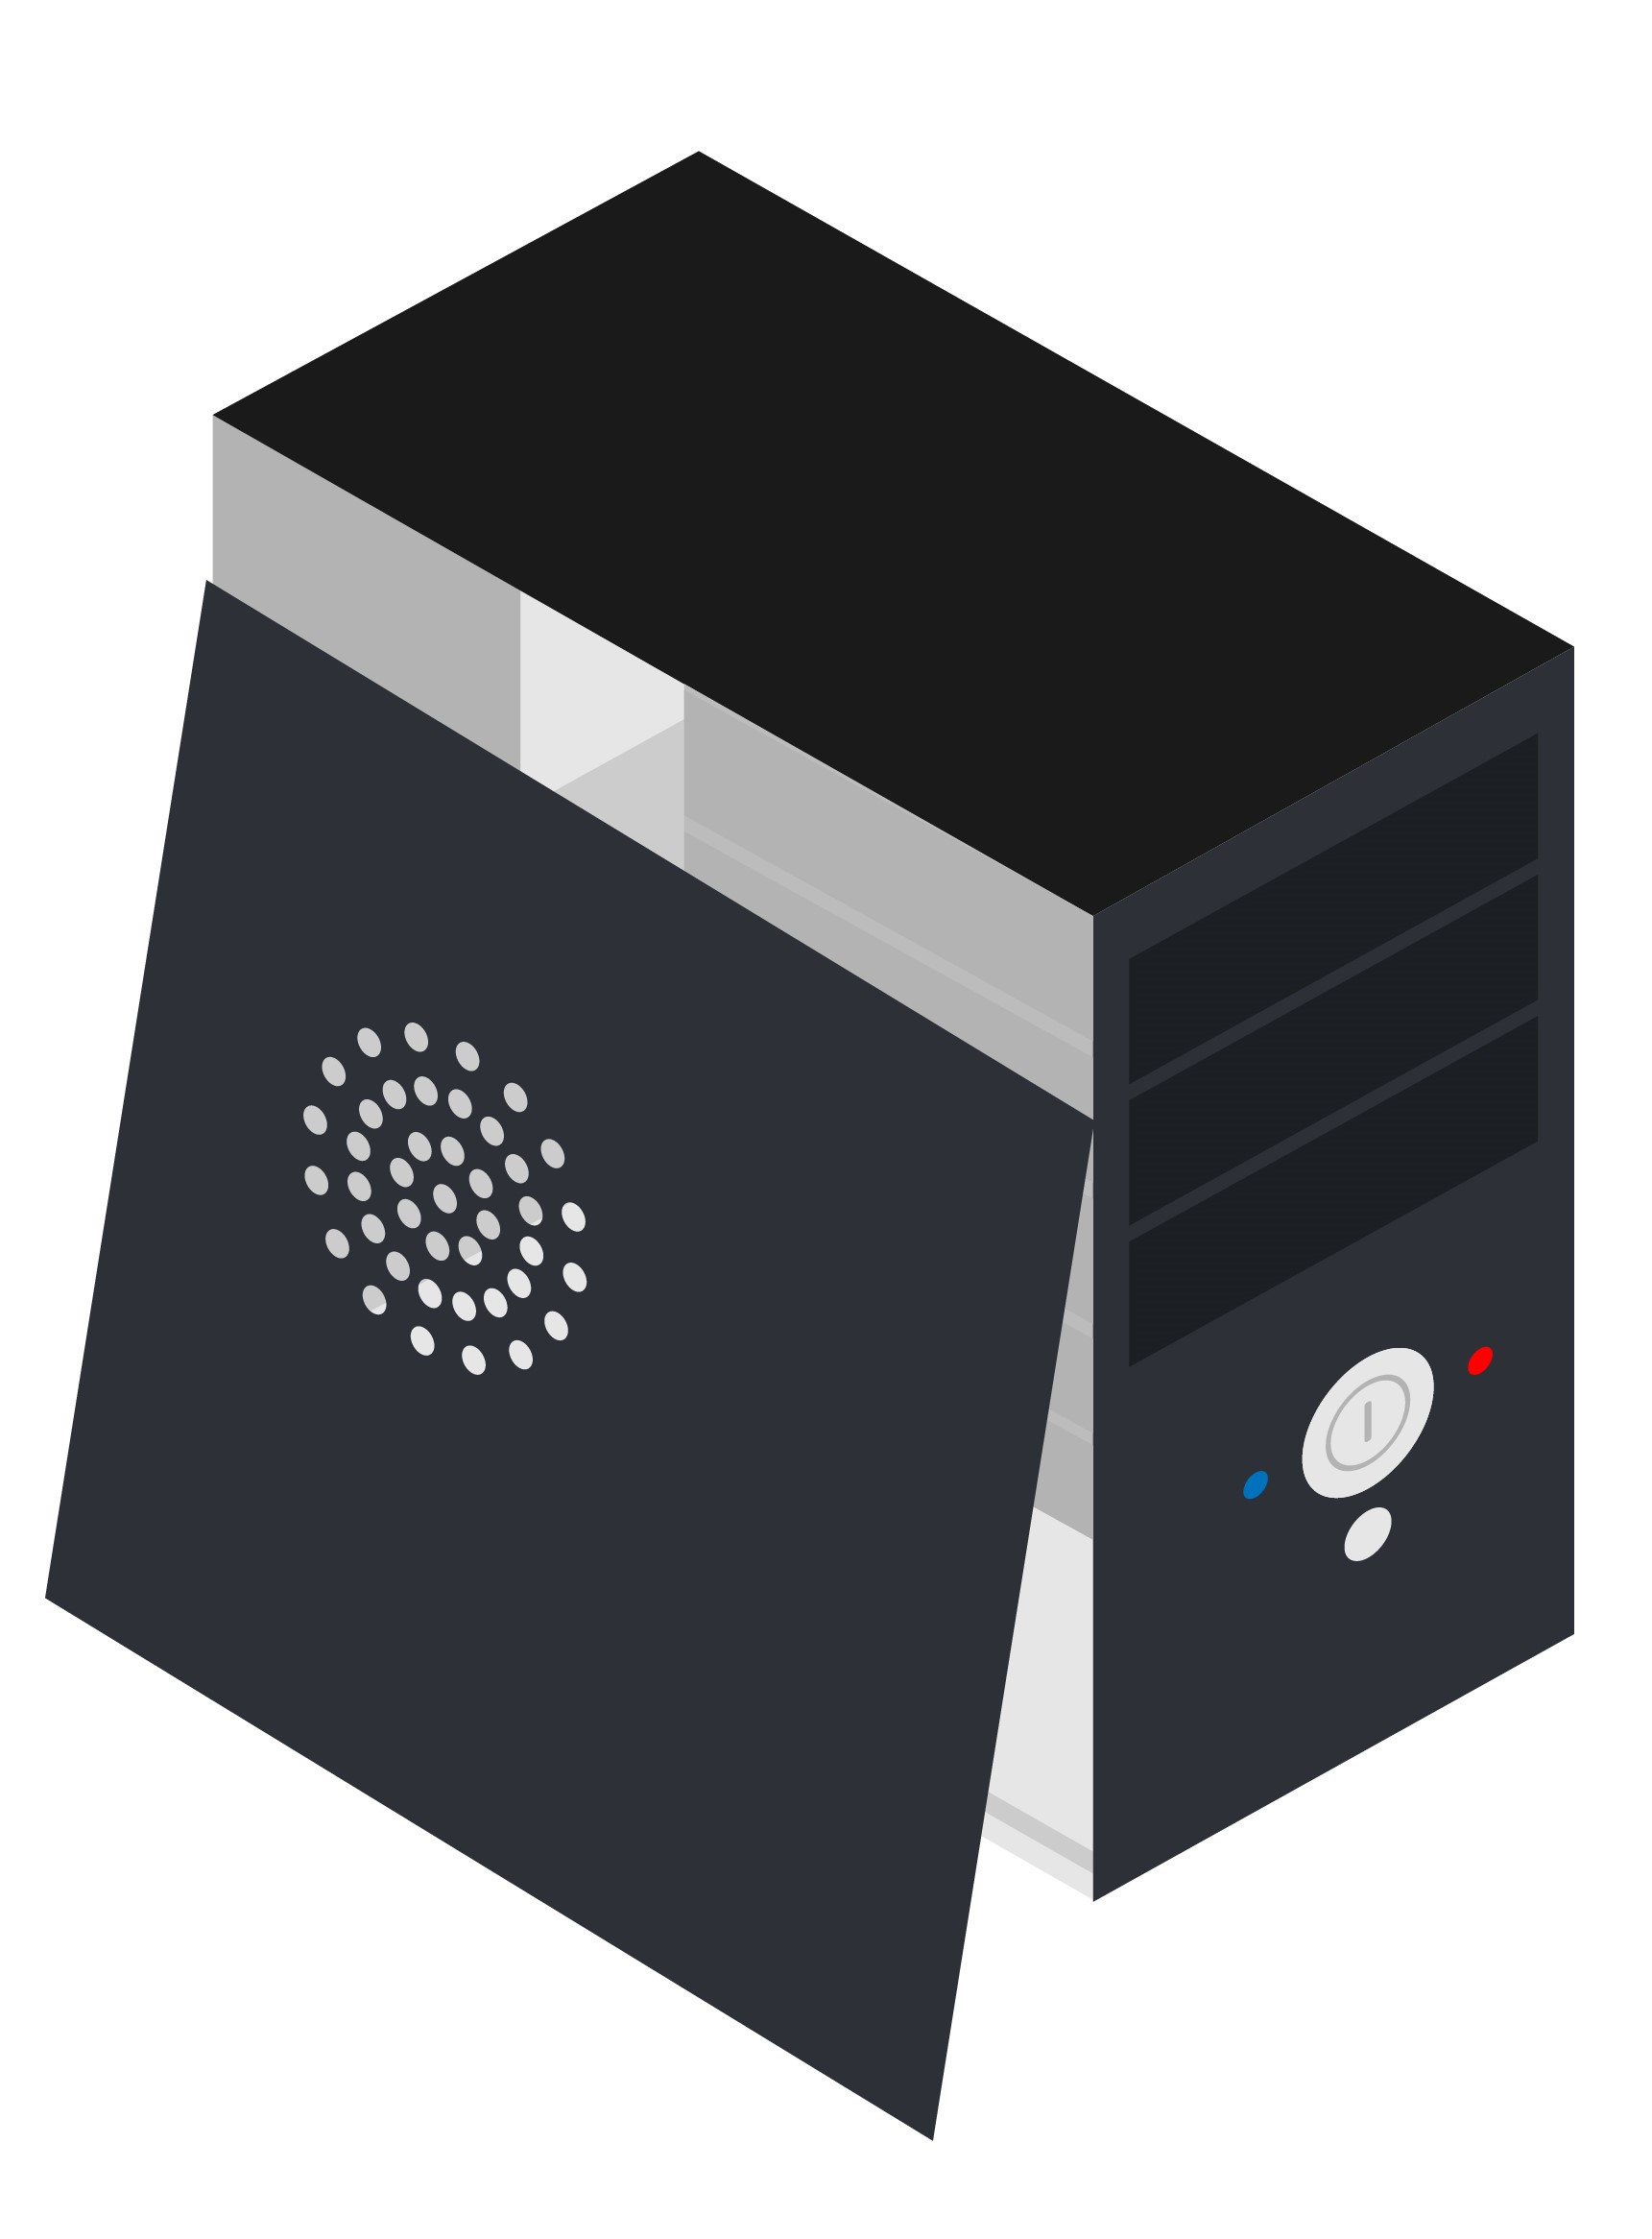
\includegraphics[width=.12\textwidth]{Simulation_sayem/pictures/casing.jpg}};
\node<1->[inner sep=0pt] (PSU) at (6,3)
    {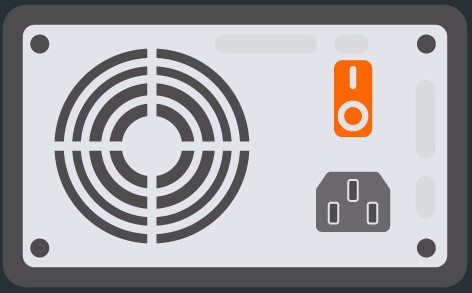
\includegraphics[width=.12\textwidth]{Simulation_sayem/pictures/powerSupply.jpg}};
\node<1->[inner sep=0pt] (CPU) at (0,3)
    {
\includegraphics[width=.08\textwidth]{Simulation_sayem/pictures/processor.jpg}};


\node<2->[inner sep=0pt] (motherboardtik) at (3,0)
    {
\includegraphics[width=.09\textwidth]{Simulation_sayem/pictures/tik.png}};
\node<3->[inner sep=0pt] (CPUtik) at (0,3)
    {
\includegraphics[width=.09\textwidth]{Simulation_sayem/pictures/tik.png}};
\node<4->[inner sep=0pt] (videocardtik) at (3,3)
    {
\includegraphics[width=.09\textwidth]{Simulation_sayem/pictures/tik.png}};
\node<5->[inner sep=0pt] (PSUtik) at (6,3)
    {
\includegraphics[width=.09\textwidth]{Simulation_sayem/pictures/tik.png}};
\node<6->[inner sep=0pt] (casingtik) at (6,0)
    {
\includegraphics[width=.09\textwidth]{Simulation_sayem/pictures/tik.png}};
\node<7->[inner sep=0pt] (memorytik) at (0,0)
    {
\includegraphics[width=.09\textwidth]{Simulation_sayem/pictures/tik.png}};

\draw<1-> [inactive edge] (videocard) --(PSU);
\draw<1-> [inactive edge] (motherboard) --(videocard);
\draw<1-> [inactive edge] (CPU) --(videocard);
\draw<1-> [inactive edge] (motherboard) --(CPU);
\draw<1-> [inactive edge] (PSU) --(casing);
\draw<1-> [inactive edge] (motherboard) --(casing);
\draw<1-> [inactive edge] (motherboard) --(memory);


\end{tikzpicture}
\end{figure}
\end{textblock}


\begin{textblock}{14}(1,11)
    \begin{itemize}
        \item<2-> Our shopping list
    \end{itemize}
\end{textblock}


\begin{textblock}{14}(2.5,12)
    
    
    \begin{tikzpicture}

\node<2->[inner sep=0pt] (motherboard) at (0,0)
    {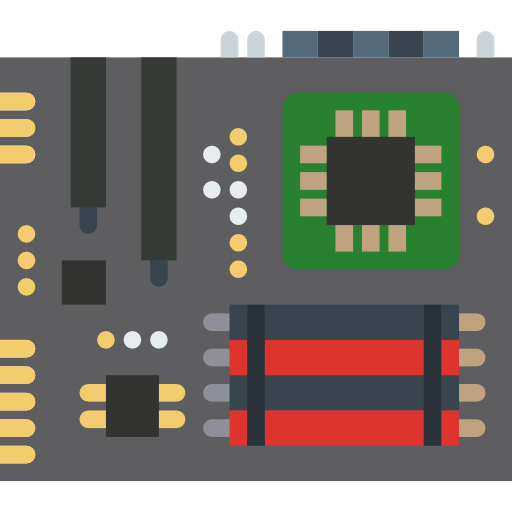
\includegraphics[width=.10\textwidth]{Simulation_sayem/pictures/motherboard.png}};  
\node<4->[inner sep=0pt] (videocard) at (4,0)
    {
\includegraphics[width=.10\textwidth]{Simulation_sayem/pictures/video-card.png}};
    
\node<7->[inner sep=0pt] (memory) at (10,0)
    {
\includegraphics[width=.10\textwidth]{Simulation_sayem/pictures/memory.png}};
    
\node<6->[inner sep=0pt] (casing) at (8,0)
    {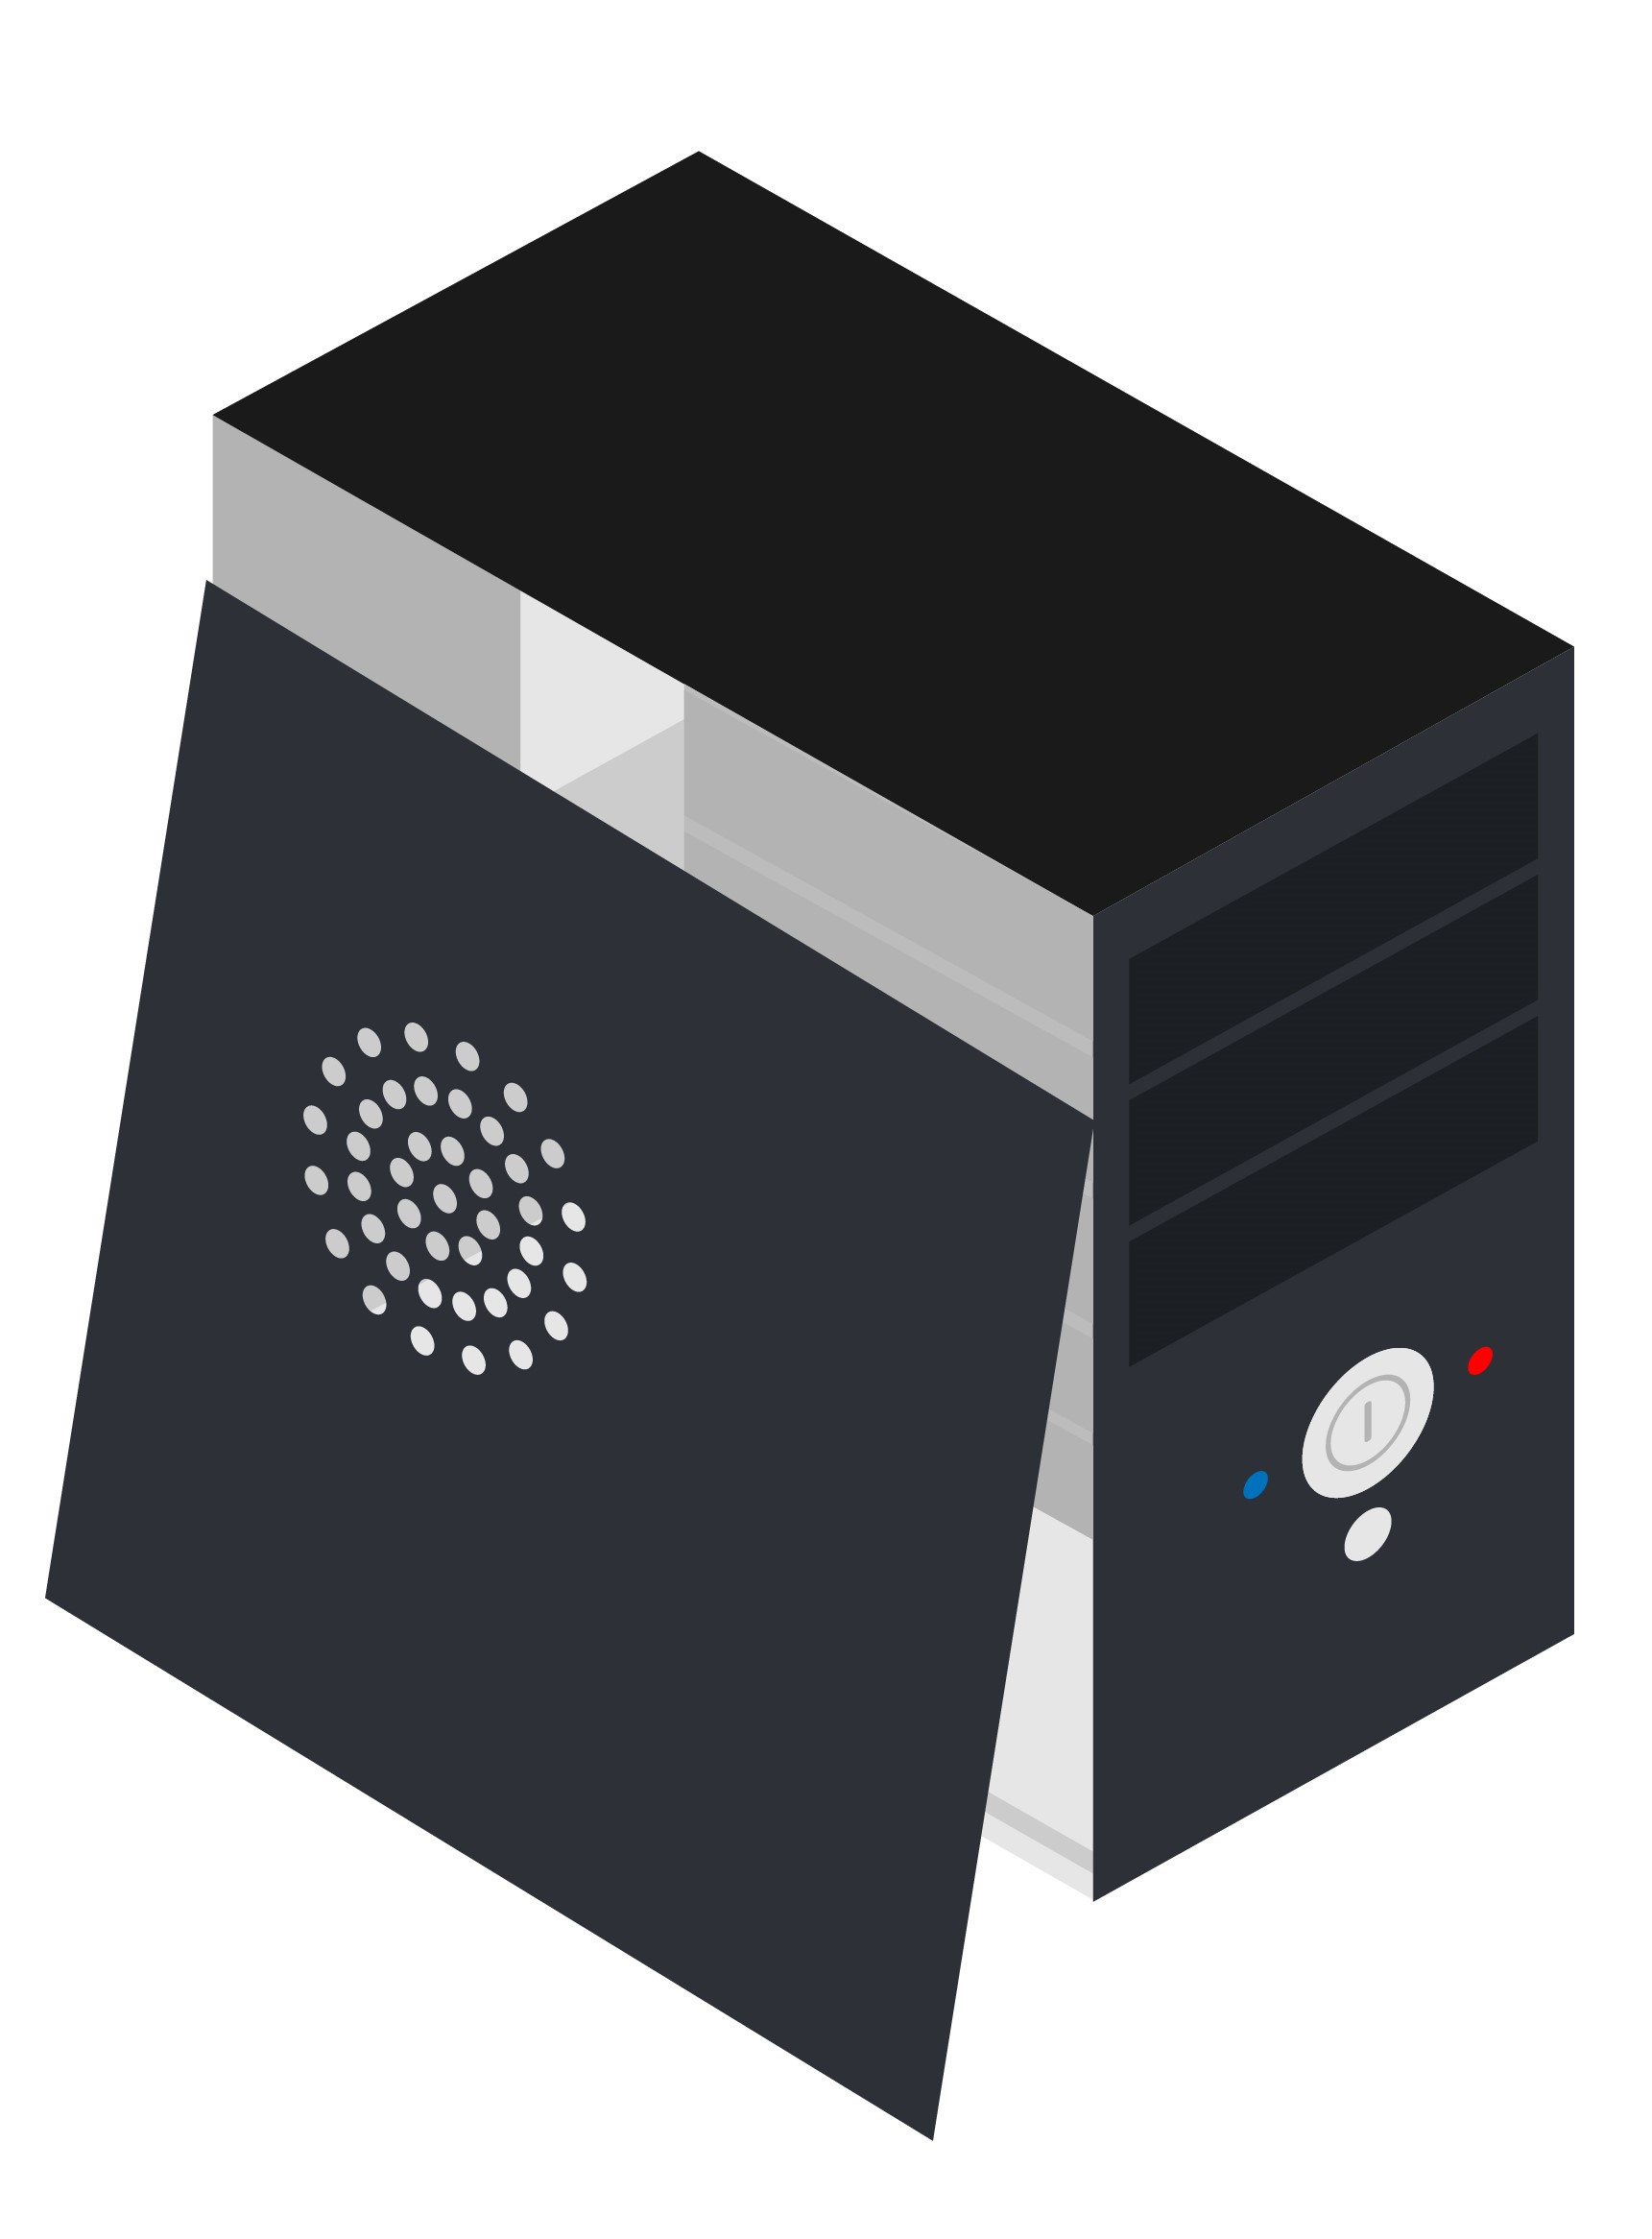
\includegraphics[width=.073\textwidth]{Simulation_sayem/pictures/casing.jpg}};
\node<5->[inner sep=0pt] (PSU) at (6,0)
    {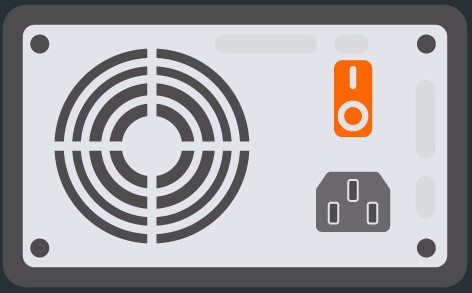
\includegraphics[width=.10\textwidth]{Simulation_sayem/pictures/powerSupply.jpg}};
\node<3->[inner sep=0pt] (CPU) at (2,0)
    {
\includegraphics[width=.06\textwidth]{Simulation_sayem/pictures/processor.jpg}};



\end{tikzpicture}

\end{textblock} 
\end{frame}


\begin{frame}
    \transfade
    

\begin{textblock}{14}(2,3)
    \begin{itemize}
    \item<1-> There can exist multiple ordering
\end{itemize}
\end{textblock}




\begin{textblock}{14}(2.5,4)
    
    
\begin{tikzpicture}

\node<2->[inner sep=0pt] (motherboard) at (0,0)
    {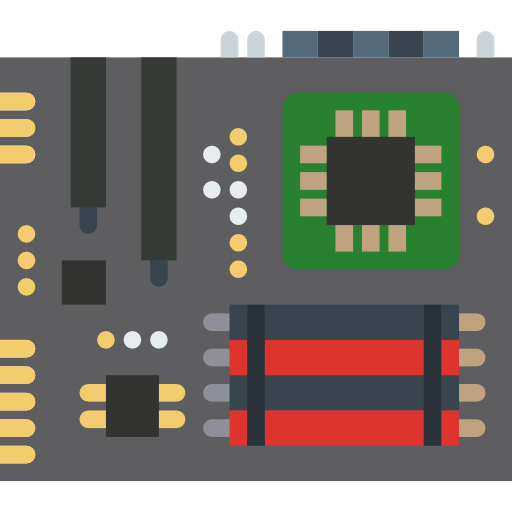
\includegraphics[width=.10\textwidth]{Simulation_sayem/pictures/motherboard.png}};  
\node<2->[inner sep=0pt] (videocard) at (6,0)
    {
\includegraphics[width=.10\textwidth]{Simulation_sayem/pictures/video-card.png}};
    
\node<2->[inner sep=0pt] (memory) at (2,0)
    {
\includegraphics[width=.10\textwidth]{Simulation_sayem/pictures/memory.png}};
    
\node<2->[inner sep=0pt] (casing) at (10,0)
    {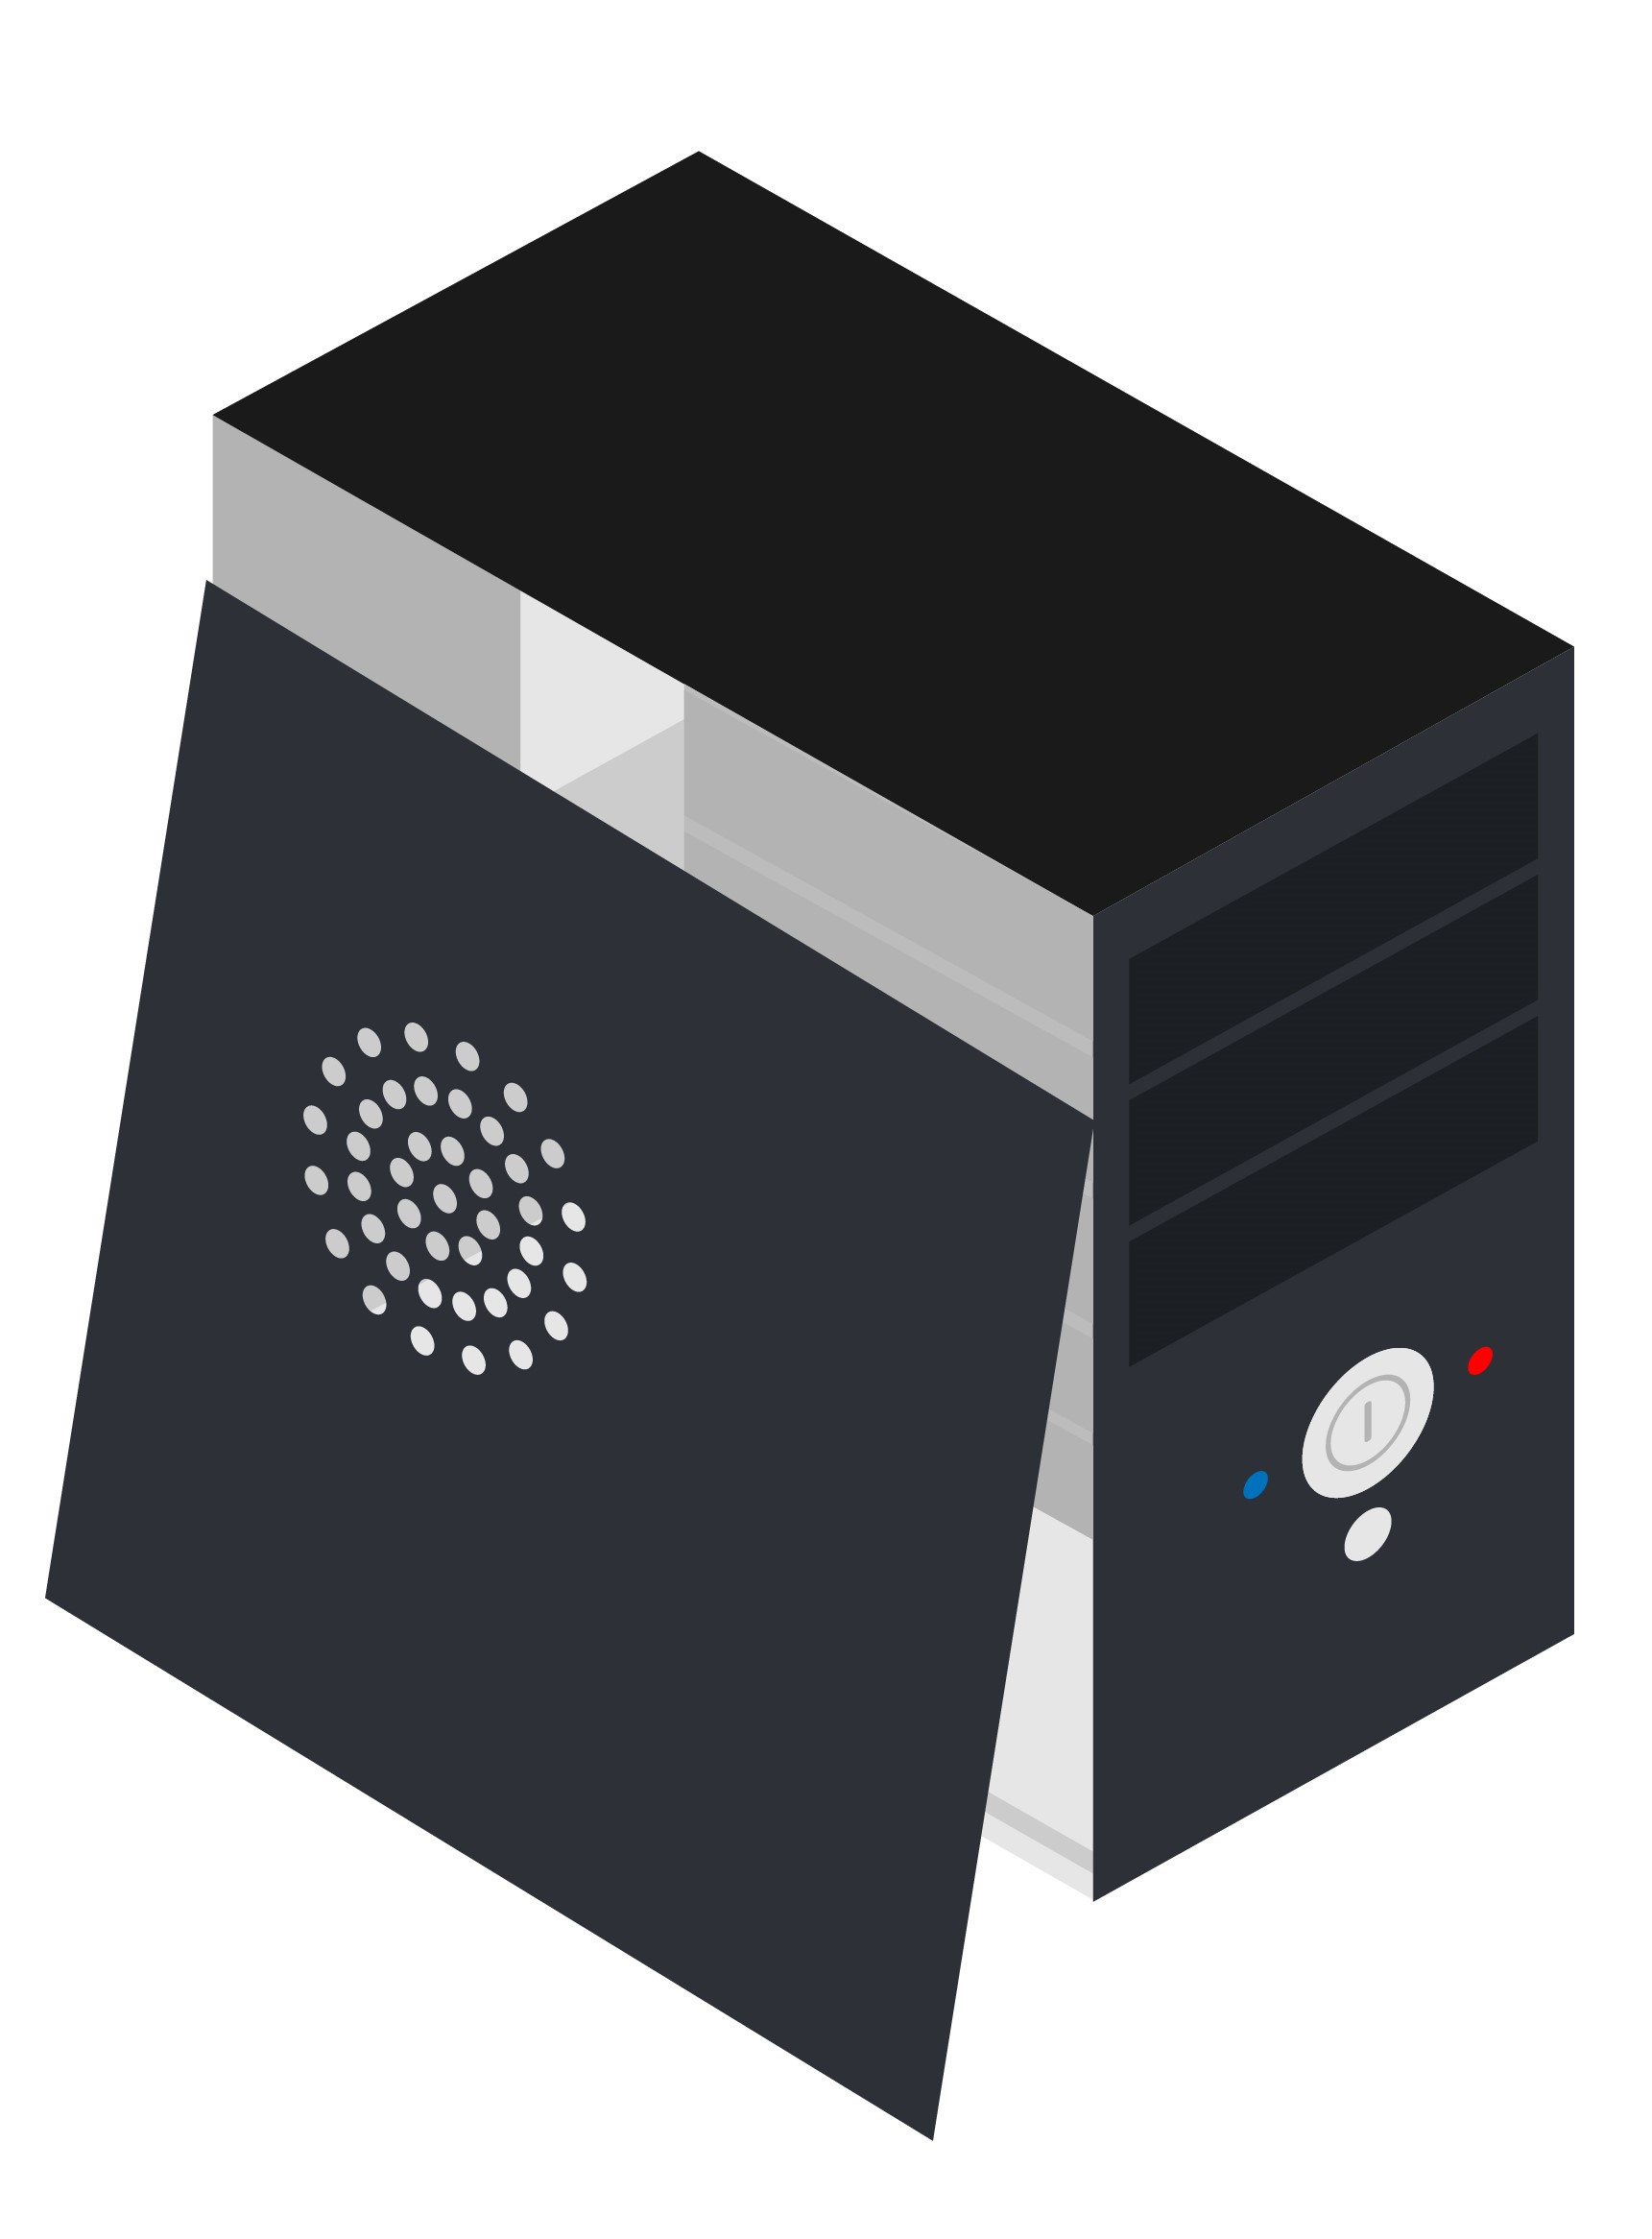
\includegraphics[width=.10\textwidth]{Simulation_sayem/pictures/casing.jpg}};
\node<2->[inner sep=0pt] (PSU) at (8,0)
    {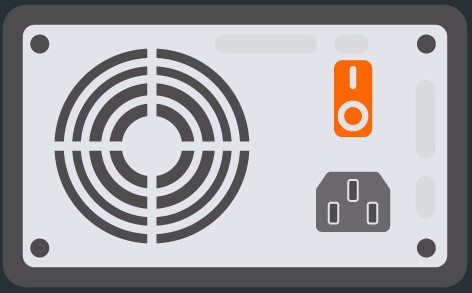
\includegraphics[width=.10\textwidth]{Simulation_sayem/pictures/powerSupply.jpg}};
\node<2->[inner sep=0pt] (CPU) at (4,0)
    {
\includegraphics[width=.06\textwidth]{Simulation_sayem/pictures/processor.jpg}};

\end{tikzpicture}

\end{textblock}


\begin{textblock}{14}(2,7)
    \begin{itemize}
        \item[]<2->RAM can be bought right after motherboard
    \end{itemize}
    

\end{textblock}




\begin{textblock}{14}(2,9)
    \begin{itemize}
    \item<3-> Dependencies should be taken care beforehand \\
    In our example, we could not buy casing before motherboard and PSU
\end{itemize}
\end{textblock}

    
\end{frame}



\begin{frame}
    \transfade
    \begin{textblock}{16}(0,7.5)
        \centering
        \color{black}
        \Large \textbf{We have used topological sorting. But how it works!!!}
    \end{textblock}
    
\end{frame}





% \begin{frame}{}
%     \transboxin
    
%     \begin{itemize}
%         \item[$\blacksquare$] Topological sort is a graph traversal in which each node is visited only after all its dependencies are visited. \underline{If there is an edge from node u to v, then v is dependent on u}  \href{https://www.interviewcake.com/concept/java/topological-sort}{\underline{Link}} \pause
%         \item[$\blacksquare$] We can view a topological sort of a graph as an ordering of its vertices along a horizontal line so that all directed edges go from left to right. Topological sorting is thus different from the usual kind of “sorting”
%         \item[$\blacksquare$] In order to have a topological sorting, the graph must not contain any cycles and it must be directed i.e. the graph must be a DAG. \pause
%         \item[$\blacksquare$] There can be more than one topological sorting for a graph. \pause
%     \end{itemize}    
% \end{frame}
